\documentclass{article}
% \usepackage[utf8]{inputenc}
\usepackage{caption}
\usepackage{subcaption}
\usepackage{graphicx}
\usepackage{emoji}
\usepackage{hyperref}
\usepackage{multirow}
\usepackage[table,xcdraw]{xcolor}

\title{\emoji{pinched-fingers} and its meanings: An emojical study \\ \normalsize{CSS Lab Holiday Paper Series 2021}}
\author{Anna Di Natale, Emma Fraxanet, Max Pellert, Jana Lasser,\\ Hannah Metzler, Alina Herderich, Segun Aroyehun, Apeksha Shetty,\\ David Garcia}
\date{\today}

\begin{document}

\maketitle

Non-verbal communication is not easy, but Italians are somehow better at it. See this video of a little Italian girl as an example: \url{https://www.youtube.com/watch?v=Z5wAWyqDrnc}. In this paper of the Computational Social Science Lab Holiday Paper Series, we set out to learn about non-verbal, non-facial communication online through the use of one of the most iconic Italian expressions: \emoji{pinched-fingers}. We study its meaning in multilingual Twitter datasets and its association with sentiment to develop a tool to help using hand emoji in online communication. We further study the role of skin color in hand emoji in Reddit and the change in their frequency of use since the beginning of the COVID-19 pandemic, as an example of an \emph{emojical study} focusing on various aspects of the use of \emoji{pinched-fingers}.


Emojis offer the possibility of new non-verbal expression online. Without having to rely on pictures or videos, we can encode our facial expression and hand gestures in text.
Over recent years, the frequency of emojis in online communication has been growing steadily, for example with tweets containing emojis reaching a 20\% rate in 2020 \cite{Emojipedia}. As new emojis are added to include offline gestures, some cultures use them with different meanings as others. Furthermore, gestures can have a meaning in a culture and be adopted by another culture through online text communication, creating a novel kind of online assimilation of non-verbal signs.

One of the newest and most confusing emojis is \emoji{pinched-fingers}, a typical Italian gesture but with other meanings and uses in other languages. The pinched-fingers emoji, as it was named by the Unicode Consortium when debuted in March 2020, was supposed to graphically represent the exasperated expression ``what do you want?", since this is the common meaning of this hand gesture when made by Italians. Its creators submitted a proposal \cite{Unicode} supporting the need for such an emoji, basing their arguments on the uniqueness and completeness of such a gesture, together with its high frequency of usage in the large group of Italian-speakers and people with Italian cultural affinity or ancestry. Finally, their proposal was accepted in 2020, together with another hundred new emojis. However, a conversation around other possible meanings of this gesture rooted in other cultures and languages pointed out that it can also mean ``wait a minute" in Israel and in the Arab world or represent an iconic gesture of the famous K-pop star, Yuri. 

Here\footnote{This paper is the result of an unofficial workshop we titled ``how not to suck handling emojis in our research".}, we study the meanings of \emoji{pinched-fingers} by analyzing Twitter data to identify the contexts in which it appears. We consider various languages to detect the drivers of its use in the events of recent years. We continue by studying the sentiment associated with \emoji{pinched-fingers} and design a NLP tool to help non-native-hand-waving speakers to learn how to express themselves in emoji hand language. We then analyze how the use of general hand emojis has changed during the pandemic and how skin modifiers of hand emojis are associated with negative votes to Reddit comments.

\section{The meanings of \emoji{pinched-fingers}}

\begin{figure}
    \centering
    \includegraphics[width=\linewidth]{Plots/topicmodel/topic_models_table.png}
    \caption{Words and interpretation of the topics obtained from the Mallet LDA model. The order of the words is directly related with their relevance to the topic.}
    \label{fig:topic_model}
\end{figure}

Using the brand new historical search endpoint of the the Twitter API v2, we retrieved an exhaustive dataset of tweets in English that contain \emoji{pinched-fingers} up to 2021-11-28, ignoring retweets. To obtain a set of topics that can give a general intuition of the different uses and contexts of the emoji, we applied topic modelling with the Mallet Latent Dirichlet Allocation (LDA) algorithm in Python's Gensim package wrapper \cite{McCallumMALLET}. 

We preprocessed the text by removing stopwords, detecting bigrams, and studying the most and least frequent words. Since the quality of preprocessing tools differs across languages, we do this first exploration only with English data. Additionally, we assume that English, in contrast to other languages, can be seen as an approximation to the different uses of the emoji in other languages when the speakers of a language communicate online with general audiences by tweeting in English. As a consequence, English Twitter text might also contain the meaning which Italians associate with \emoji{pinched-fingers}. 

Another important parameter in the use of the topic model is the number of topics. We explore a large range of values and compute the coherence score for each number of topics, obtaining a maximum coherence score for a model with 24 topics. For the obtained topics, reported in Figure \ref{fig:topic_model}, we group and describe the diverse contexts in which we encounter the ``unique" (or not so much) Italian emoji. We also take into account examples of tweets that represent each topic, and compare with a smaller model with 15 topics that summarizes better some groups of topics.

The first three topics are related to Italian culture: Topic 1 is a direct representation of Italian culture and language and its relation to hand gestures and emojis. Topic 2 and Topic 3 are related to food and sports, specifically to Italian gastronomy and sport events in which Italy was heavily involved (e.g., they won the UEFA Euro 2020). Secondly, Topic 4 shows a strong connection to politics, which could be linked to complaints about regulations and political decisions. The next broad group of topics (5-9) is related to the concept of quality of different objects (art, movies, music...). The fact that the expression the ``chef's kiss" appears in these topics hints that \emoji{pinched-fingers} may express appreciation for good quality and excellence in these tweets. Next, we surprisingly find a topic related to cryptocurrency, in which \emoji{pinched-fingers} could mean holding a investment in cryptocurrency for future profits. We further observe a topic that we interpret as spam-related tweets, which make use of a large number of emojis to attract attention. An example of a fictional tweet that combines these two topics would be the following: \emph{``We just minted an NFT of \emoji{pinched-fingers} and put it for sale for the affordable price of 100 ETH!! Buy it now here: \url{https://bit.ly/3q4IEUQ}"}\footnote{We promise we will use the earnings of this NFT for future research.}.
    
Another surprising finding is that K-pop fandoms (or fan groups), such as Army (BTS fan group), dominate part of the usage of this emoji. Studying some of these tweets individually revealed that \emoji{pinched-fingers} can be used to replace the finger-heart gesture. The K-pop industry popularized this gesture in South Korea around the 2010s. It still does not have an official emoji, despite the strong presence of K-pop topics online. However, a new emoji for the finger-heart gesture will be released in the upcoming 2022 official emoji update. It would be interesting to study whether this context of \emoji{pinched-fingers} still appears a while after this release, or if its meaning finally returns its original one. 
Two further well-defined topics relate to negative emotions. The first includes insults in general and the second one is particularly linked to stress due to school or university deadlines, and possibly includes complaints. The other topics found in this classification were not easily interpretable, and dissolved into the topics described above when the model was set to 15 topics. We chose the version of 24 topics due to its higher coherence score and because we like it and this is a Holiday Paper Series article after all.

\section{Differences across languages}

Thanks to the new counts endpoint of the Twitter API v2, we can track the frequency of an emoji within a language over time. We calculated the daily count of tweets in six languages (English, German, Spanish, Italian, Japanese, and Korean) that contain \emoji{pinched-fingers}, dividing the count over a baseline that we estimated with the daily count of tweets in those languages that contain at least one stopword. We excluded retweets in all these counts to measure frequency of expression and not in sharing text. We then smoothed the daily counts with a seven-day rolling average. Figure \ref{fig:freq_pinchedfingers} shows the time series for Italian, English, and Korean with spikes highlighted. Using our access to Brandwatch, we generated word clouds including retweets\footnote{We know that wordclouds are the pie charts of text analysis, but we didn't have time to make anything fancier. And we like them after all.} on the peaks to get an idea of the words driving the increase in use of \emoji{pinched-fingers}.

\begin{figure}[hbtp]
\centering
  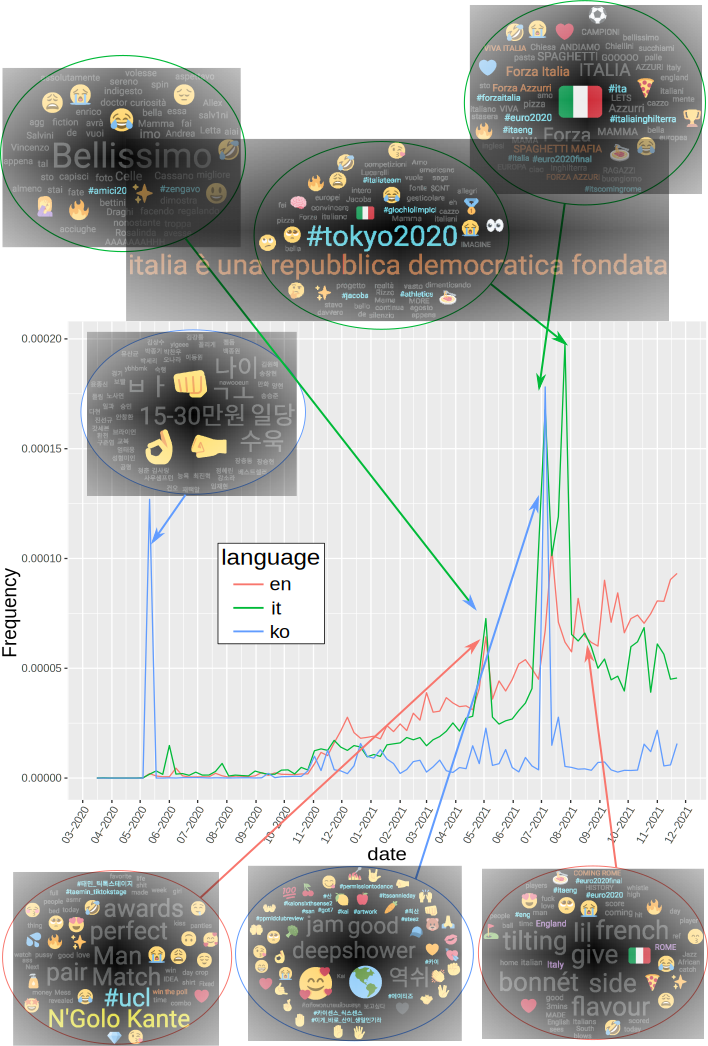
\includegraphics[width=1\linewidth]{Plots/freq_wordclouds-vertical.pdf}
\caption{Frequency of usage of \emoji{pinched-fingers}. Peaks are reported together with the relative wordclouds. The frequencies are plotted starting from March 2020 when the emoji was introduced.}
\label{fig:freq_pinchedfingers}
\end{figure}

The first Italian spike is driven by users complaining about politics and the big brother TV show ('gf' stands for grande fratello, where Rosalinda is one participant). The second peak is related to the final match Italy vs England in the soccer Euro Cup. Here, the English hashtag \#itscominghome referring to the cup was dubbed into \#itscomingrome. Note how terms associated with Italians (both iconic behavior and stereotypes) are also used by Italian speakers (pizza, pasta, spaghetti, even mafia). The third spike is related to the Italian successes in the Olympic games, especially to the winner of the men's 100m run, the Italian Jacobs. The enthusiasm about the Italian sportive successes, together with Italians making fun of themselves, is rendered in this popular tweet: \url{https://twitter.com/gocciodigin/status/1421835234023202818}. As we saw, the pinched fingers in Italian are used in tweets about the Euro 2020 football cup and the Olympics of Tokio 2020, showing its connection to national pride.

The first spike in English relates to a match of the UEFA Champions League (UCL). We didn't manage to understand the association between this event and \emoji{pinched-fingers}. The second spike in English also relates to the final match of Euro 2020, including the reference to \#itscomingrome. 

The first peak in Korean is driven by viral and spam-like tweets about money, using the meaning of \emoji{pinched-fingers} about money or wealth (as in holding a coin). The second Korean peak is linked to a song by the Korean DJ Deepshower, where \emoji{pinched-fingers} is used with the meaning of ``quality". In Korean, \emoji{pinched-fingers} is associated to many other hands emojis (see word clouds), while in Italian and English it is not.

A closer inspection of the wordclouds in Figure \ref{fig:freq_pinchedfingers} shows different kinds of sentiment for different languages. To test this, we classified the tweets including the emoji at least once with a multi-lingual XLM-RoBERTa model fine-tuned for sentiment classification \cite{barbieri2021xlmtwitter}, which was trained on mostly on languages written in Latin characters. Figure \ref{fig:sentiment} shows the fractions of tweets classified as positive, negative, and neutral across languages. We can see that the most positive language is Japanese, followed by Turkish and French. We identified many positive French tweets where  \emoji{pinched-fingers} is related to quality, especially in the context of food. The most negative languages in the context of \emoji{pinched-fingers} are Spanish and Italian, referring to the meaning of exasperation that motivated the initial proposal of including the emoji in the Unicode standard.


\begin{figure}
    \centering
    \includegraphics[width=.8\linewidth]{Plots/sentiment.png}
    \caption{Distribution of sentiment of Tweets containing \emoji{pinched-fingers} across languages.}
    \label{fig:sentiment}
\end{figure}

\section{Emoji tech: helping with emojical expression}

For potential funding reasons, we also address the burning question of how Information and Communications Technologies can enable people to have better experiences with hand emojis in Italian by advising them on situationally-aware hand reactions. Our integrated, interactive, computationally-assisted approach is exclusively validated on synthetic, complimentary, native and non-native speaker examples \footnote{Our buzzword sentence generator broke when producing this text}. We came up with as many examples as we could  without being distracted too much from other work tasks like planning an office Christmas party, which was then cancelled because of the restrictions related to the COVID-19 pandemic. This makes it a strong candidate for high performance on benchmark tasks (to be developed in a series of papers later) and of very little relevance outside of this stylized domain, as it is common in many Machine Learning scenarios. In short, we substantially contribute to the current paradigm in NLP research but also contribute to the social sciences: Our approach is also grounded in deep theory, we promise.\footnote{On request, we also share Zotero libraries of 1000s of papers for intimidation purposes.}

We use BERTino \cite{muffoBERTinoItalianDistilBERT2020}, a large-scale model pretrained on Italian text and fine-tune it on the FEEL-IT emotion classification dataset \cite{bianchi-etal-2021-feel}. Our emotion classifier\footnote{The model is available from the authors on unreasonable request.} can detect 4 discrete emotions: joy, fear, anger and sadness. We combine the three negative emotions to one general negative class and map joy to positive. The preprocessing of the text cleaned it of many words that can not be legally passed as inputs to Italian language models because of blasphemy laws. BERTino-feel-it allows us to feed any Italian text into it and to recommend a fitting hand emoji to be added to the text. It produces the following (stereo)typical examples:
\begin{itemize}
    \item ``Odio il modo in cui la regione vicina prepara il piatto"/``I hate the way the neighboring region is preparing the dish". Our classifier rightly sees the anger here and recommends the following emoji:
\emoji{pinched-fingers}

\item ``L'Italia è super campione del mondo in tutti gli sport"/``Italy is the super world champion in every sport". The joy and national pride contained in this sentence is correctly translated into \emoji{ok-hand}.

\item ``Non apriamo prima di mezz'ora, non importa cosa dice il cartello"/``We don't open for another half hour, no matter what the sign says". This example shows that our classifier is also able to capture fine-grained nuances of emotional expression in natural languages by choosing \emoji{middle-finger}.
\end{itemize}

\section{Hand and face emoji after mask mandates}

During the COVID-19 pandemic, many countries have introduced several kinds of mask mandates, making masks a very usual sight in our everyday offline interactions. This reduces expressive power in facial non-verbal expression, making it harder to communicate through smiles or other signs that are partially or completely covered by masks. In our everyday life, we noticed that some of us use our hands more to communicate when using a mask, for example to express approval or disapproval. This is especially useful when masks muffle verbal expression or in very noisy environments. We thought that this could have an effect in how we choose emojis online: is it possible that hand emojis became more frequent over time compared to face emojis since the beginning of mask mandates during the COVID-19 pandemic?

Using the counts endpoint of the Twitter API v2, we counted the frequency of several hand emojis and facial expression emojis. We excluded the new emojis that appeared after the beginning of 2019 from these counts. Emojis related to the pandemic, like the face with a mask emoji \emoji{face-with-medical-mask}, are included in the count of face emojis. This allowed us to calculate a frequency of hand emoji per face emoji on a weekly basis over time, in particular in the three years between December 2018 and December 2021. Figure \ref{fig:ratio} shows the weekly ratio of hand to face emojis, with a vertical line marking March 2020 as the moment when COVID-19 was declared a pandemic. You can see a change in the frequency of hand to face emojis, from values below 0.4 during 2019 to values closer to 0.45 in 2021. Note that we find this pattern considering all emojis, also the ones related to the pandemic, but the results are similar when excluding pandemic-related emojis like \emoji{face-with-medical-mask} and \emoji{face-with-thermometer}.

\begin{figure}[hbtp]
    \centering
    \includegraphics[width=0.9\linewidth]{Plots/ratio_all_weekly.png}
    \caption{Ratio of hand emojis to face emojis on the 6 languages considered. The blue line indicates a linear model fitted on the data prior to January 2020. The red line indicates the moment when COVID-19 was declared a pandemic. Counts are aggregated on a weekly frequency.}
    \label{fig:ratio}
\end{figure}

To test if the pandemic has increased the relative frequency of hand to face emojis on Twitter, we fitted a linear model of the trend of this ratio with data prior to January 2020 and extrapolated after the beginning of the pandemic. The blue line in the figure shows the prediction trend, which is substantially below the actual value of the ratio afterwards. This observation is consistent across languages too. We computed the model and measured the mean residual of the model in its extrapolation since March 2020 as a measure of the effect of the pandemic on this ratio. Table \ref{tab:lm_hoverf} reports the effect for the six languages we considered, both in terms of mean residual and as a percentage increase over the previous hand to face emoji ratio. You can see that the effect is heterogeneous across countries, with some experiencing large increases (e.g. English with 24\% and Korean with 39\%) but with Japan experiencing no significant increase. All increases were significant in t-tests except for Japanese, as in Japan the use of face masks in public was more frequent before the pandemic than in other countries.



\begin{table}[hbtp]
    \centering
    \begin{tabular}{|c|c|c|}
    \hline
    Language & mean residual & percentage\\
    \hline
        Italian & 3.26*10$^{-4}$ & 15\% \\
        \hline
        German & 5.60*10$^{-4}$ & 22\%\\
        \hline
        Spanish & 4.63*10$^{-3}$& 8.4\%\\
        \hline
        Korean & 5.63*10$^{-3}$& 39\%\\
        \hline
        Japanese & 2.31*10$^{-4}$&0.2\% \\
        \hline
        English & 4.53*10$^{-2}$& 24\% \\
        \hline
        All & 5.67*10$^{-2}$ & 14\%\\
        \hline
    \end{tabular}
    \caption{Mean residuals of the prediction model for the frequency of hand emojis in 2019 computed on data from 2020 and 2021. P-values of the t.test are all $<10^{-5}$ apart from Japan, which has $p=0.8$.}
    \label{tab:lm_hoverf}
\end{table}

\section{Not all hands are equal on Reddit}

Hand emojis can be adapted with skin color modifiers to match the skin of the person using them. Unlike other emojis, where only a small area is affected by the skin modifier, hand emojis change in color as they mainly show the skin of a hand. On Reddit, the subreddit r/shitposting\footnote{Visit this subreddit at your own risk. It is full of politically incorrect memes and can contain NSFW content.} had a running meme of how the darkest thumbs up emoji gets downvoted in comments in comparison to other skin colors of the same emoji\footnote{\url{https://www.reddit.com/r/shitposting/comments/r5peim/racism/}}. Based on this observation, we test the \emph{shitposting hypothesis:} comments on Reddit with dark skin emoji modifiers are more likely to have a negative score than comments with the same emoji but without the skin modifier or with light skin colors.

We analyzed the Reddit comments dataset of Pushshift.io\footnote{\url{https://files.pushshift.io/reddit/comments/}} \cite{Pushshift} for one year between July 2020 and June 2021. We found 3,306,680 comments (in any language) with \emoji{thumbs-up} regardless of skin modifier. To test the shitposting hypothesis, we fitted a logistic regression model with a dependent variable that takes value one if the comment had a negative Reddit score (more negative votes than positive votes) or zero otherwise. As independent variables, we coded binary variables that take the value 1 if a skin color emoji is modifying the \emoji{thumbs-up} emoji in the comment. The result of the model can be seen on the left panel of Figure \ref{fig:Skin1}, where we show the predicted probabilities of a comment having a negative score for the cases of containing at least one emoji of each skin color. We find that the darkest skin tone is associated with approximately double probability of having a negative score than the other skin colors, which don't substantially differ in their skin probability. It appears that this result agrees with the hypothesis: a comment with \emoji{thumbs-up-dark-skin-tone} is substantially more downvoted than one with other modifiers. 

\begin{figure}[h!]
    \centering
    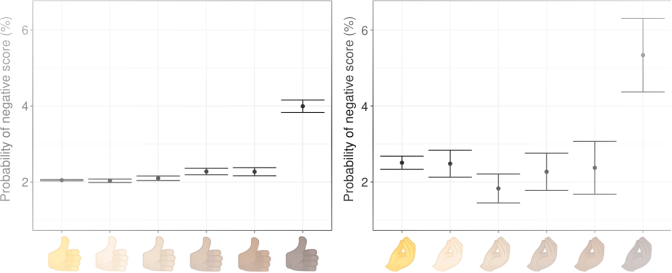
\includegraphics[width=0.9\linewidth]{Plots/Shitposting.pdf}
    \caption{Predicted probability of a Reddit comment having a negative score in the logistic regression model of skin color modifiers for comments with \emoji{thumbs-up} (left) and with \emoji{pinched-fingers} (right). Error bars show 95\% Confidence Intervals.}
    \label{fig:Skin1}
\end{figure}

We repeated the above analysis for comments in the dataset that contain \emoji{pinched-fingers}, finding 49,025 comments in total. The results of the same model are shown on the right panel of Figure \ref{fig:Skin1}, revealing a similar pattern as for \emoji{thumbs-up}: the probability of receiving a negative score is similar across skin colors but jumps to nearly double the value for the darkest skin color.

To explore how generalizable this effect is across all emojis, not just hand emojis but also ones including faces, we repeated the analysis over a sample of 120 Million Reddit comments including all comments and coding the case in which there is no skin modifier at all. The result is shown in Figure \ref{fig:Skin2}. As in the cases of \emoji{thumbs-up} and \emoji{pinched-fingers}, the probability of a comment having a negative score is approximately double when it contains the darkest skin color modifier as opposed to not having any skin color modifier. This large dataset allows us to see some smaller differences between skin tones, where the second lightest skin tone has the same probability as without any skin color modifier and the other three have a slightly larger probability. 

\begin{figure}[h!]
    \centering
    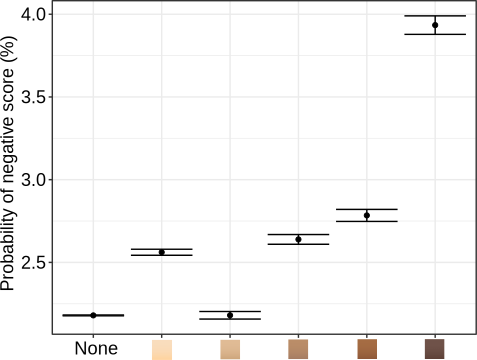
\includegraphics[width=0.6\linewidth]{Plots/FullSkinResults.pdf}
    \caption{Predicted probability of a Reddit comment having a negative score in the logistic regression model of general skin color modifiers for all emoji, not just hands. Error bars show 95\% Confidence Intervals.}
    \label{fig:Skin2}
\end{figure}


Note that the lightest modifier, especially when applied to some face emoji, generates a figure with dark hair (for example \emoji{girl-light-skin-tone}), while the second lightest generates faces with blonde hair (for example \emoji{girl-medium-light-skin-tone}). Previous research shows that the lightest modifier is used widely in East Asia \cite{Coats2018}. Describing the origins of this effect requires a more serious research paper. Please take these insights as the result of a very initial exploration on an important topic that deserves a careful analysis. Future research should try to identify if it can be attributed to racism or it could be a response to some kind of blackface behavior, despite being found to be rare on Twitter in previous research \cite{Robertson2018}. We should especially test if the effect is mostly present on some subreddits and include a language model for the rest of the text that can serve as a set of control variables to isolate the effect of the skin color modifier alone.



\section{To sum up}
\begin{itemize}
    \item We find that \emoji{pinched-fingers} can be used in various contexts, including Italian culture, K-Pop, and crypotcurrency spam.
    \item Language differences are clear too, with Japanese being the most positive language in the use of \emoji{pinched-fingers} and Spanish and Italian being the most negative.
    \item A combination of language models can be used to infer the hand emoji to add to a tweet as shown by our inspection of predictions for Italian.
    \item The fraction of hand to face emojis has increased since the beginning of the pandemic reflecting the need for hands in non-verbal expression during mask mandates, also online.
    \item Reddit comments with dark skin modifiers have approximately double the probability of getting a negative score, not just for \emoji{pinched-fingers} and \emoji{thumbs-up} but also for other uses of the skin color modifier.
\end{itemize}

Thanks for reading and all the best for 2022!

\bibliographystyle{plain}
\bibliography{bibliography}
\end{document}